\chapter{ECG: Electrocardiogram}
In this experience we built and designed an electrocardiogram and tested it on a member of the group.

\section{Materials}
\begin{itemize}
\item Instrumentation amplifier (INA) AD622
\item Precision +5V Voltage Reference REF02
\item Thermoresistor PT100
\item Resistors, trimmers
\item Power supply RIGOL DP831A
\item Waveform generator RIGOL DG1032
\item Multimeter RIGOL DM3068
\item A AD622, three OP07, a ISO124
\item Three electrodes
\item Batteries $9$ V
\end{itemize}
The resistors used were all with an uncertainty of 5\%
\section{Experimental setup}
The circuit connected with the patient was all powered by using a battery $\pm 9$.
The signal thatwe should aquire from the electrodes has a frequency of around 1.5 Hz and an amplitude of $\pm$1 mV with an offset due to the internal potential of the electrodes of 700 mV. We also need to consider the possible sources of noise caused by the movement of the body and of the cables, also by the parasitic capacitance and inductance. For these things our circuit need to remove the common potential and annihilate as much as possible the noise without removing signals at 1.5 Hz frequencies.
\begin{figure}
\centering
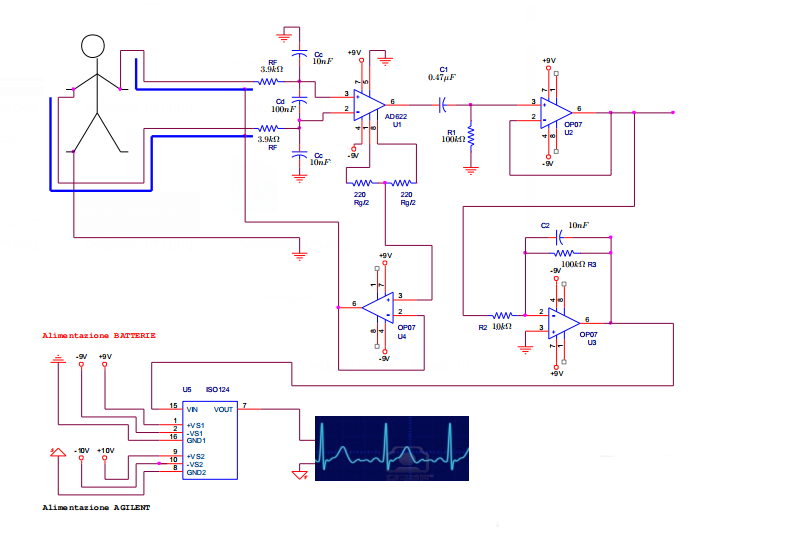
\includegraphics[width=.8\textwidth]{8/circuit.png}
\caption{Wave measured}
\end{figure}
The  first step was removing high frequency noise by using two low-pass filters on the input by using two resitors and three capacitors.
Than we removed the common signal by using the AD622 with a gain $G = \frac{50.1 k\Omega}{440 \Omega} + 1 = 116$, where at the denominator there is the resistance of the resistor connecting pin 1 and 8. This resistor is actually built with two resistors in series with half its value. The signal between these two resistors is used in a follower that serves to set the potential of the cable's shield to the same of the wire. Than we chose to put the signal amplified by the AD622 into a high-pass filter for removing other DC (or almost DC) components and than we used a follower for mismatching the impedance of the circuit. The penultimate step was taking the signal out of the follower and connecting it to a active low-pass filter.\\
The last step was decoupling the circuit connected with the patient with the circuit of the oscilloscope, by using an ISO124. This is done for physically separating the power generator and oscilloscope from the the circuit connected with the patient. This was done for avoiding electrocuting the patient in case of mulfunctions.
\section{Data analysis}
\begin{figure}[H]
\centering
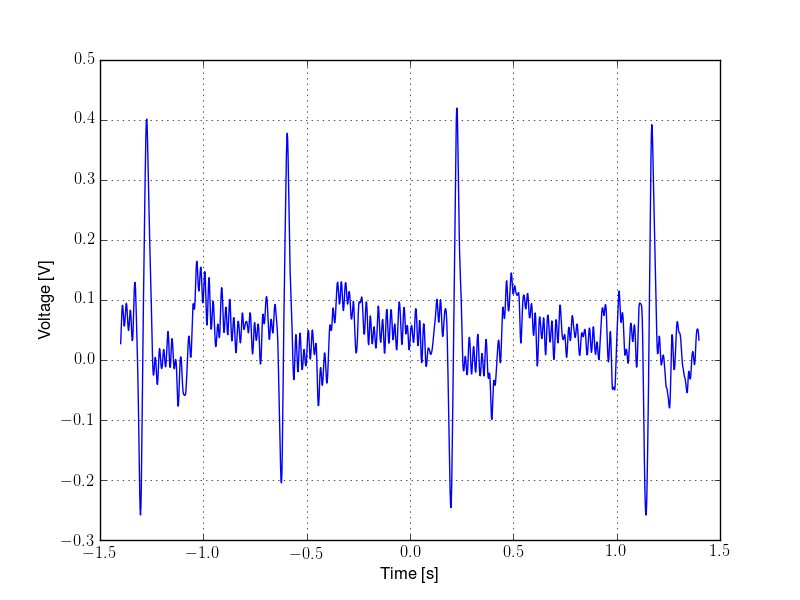
\includegraphics[width=.7\textwidth]{8/ecg.png}
\caption{Signal measured}
\end{figure}
The signal acquired with the oscilloscope is in the figure above. Originally we had noise at high frequency, the signal above is smoothed with a running mean algorithm.